
\begin{opgavetekst}{Problem 1}
\end{opgavetekst}
%
%
\begin{delopgave}{1}
	Convert the following angles from degrees to radians.
	\begin{align*}
		&1) \ 180^\circ & &2) \ -45^\circ\\
		&3) \ 20^\circ & &4) \ 180^\circ 
	\end{align*}
\end{delopgave}
\begin{delopgave}{2}
	Convert the following angles from radians to degrees.
	\begin{align*}
		&1) \ \frac{7\pi}{12} & &2) \ \frac{3\pi}{2}\\
		&3) \ -\frac{5\pi}{6} & &4) \ \frac{11\pi}{24} 
	\end{align*}
\end{delopgave}
%
%
%
%
%
\begin{opgavetekst}{Problem 2}
\end{opgavetekst}
%
%
\begin{delopgave}{1}
	Solve the following trigonometric equations on $0 \leq x \leq 2\pi$. 
	\begin{align*}
		&1) \ \cos(x)^2 = \frac{3}{4} & &2) \ (\sin(x)+1)^2 = \frac{9}{4}\\
		&3) \ 4\cos\left(x-\frac{\pi}{4}\right)^2+4 - 8\cos\left(x-\frac{\pi}{4}\right) = 4 
	\end{align*}
\end{delopgave}
%
%
%
%
%
\begin{opgavetekst}{Problem 3}
	The first two terms of a sequence $\{a_n\}$ is $a_1 = 4$ and $a_2 = 12$.  
\end{opgavetekst}
\begin{delopgave}{1}
	Determine $a_3$, $a_4$ and $a_5$ if $\{a_n\}$ is arithmetic. 
\end{delopgave}
\begin{delopgave}{2}
	Determine $a_3$, $a_4$ and $a_5$ if $\{a_n\}$ is geometric. 
\end{delopgave}
%
%
%
%
%
\begin{opgavetekst}{Problem 4}
\end{opgavetekst}
\begin{delopgave}{1}
	Determine the value of the integral
	\begin{align*}
		\int_1^{e^{\pi}} \frac{\sin(\ln(x))}{x} dx.
	\end{align*}
\end{delopgave}
%
%
%
%
%
\newpage
%
%
\begin{opgavetekst}{Problem 5}
	A function $h$ is given by
	\begin{align*}
		h(x) = 3x^2 - 4x + 7.
	\end{align*}
\end{opgavetekst}
\begin{delopgave}{1}
	Determine an antiderivative of $h$ that passes through the point $(2,20)$. 
\end{delopgave}
%
%
%
%
%
\begin{opgavetekst}{Problem 6}
	A function $f$ is given by
	\begin{align*}
		f(x) = \sin(x)x^4.
	\end{align*}
\end{opgavetekst}
\begin{delopgave}{1}
	Determine $f'(x)$. 
\end{delopgave}
\begin{delopgave}{2}
	Determine the slope of the tangent of $f$ at $x_0 = \pi$. 
\end{delopgave}
%
%
%
%
%
\begin{opgavetekst}{Problem 7}
	Let $a$ be given as $a = 0.7222\hdots$
\end{opgavetekst}
%
%
\begin{delopgave}{1}
	Write $a$ as an infinite series. 
\end{delopgave}
\begin{delopgave}{2}
	Write $a$ as a rational number. (Remember that a rational number is a fraction of two integers). 
\end{delopgave}
%
%
%
%
%
\begin{opgavetekst}{Problem 8}
	The owner of a stud wants an enclosure for horses next to the stables as seen on Figure \ref{fig:horse}.
	The enclosure should be rectangular and the owner obviously wants the enclosure to have as large an area as
	possible. The owner has 200m of fence in total for the enclosure.
	\begin{figure}[H]
		\centering
		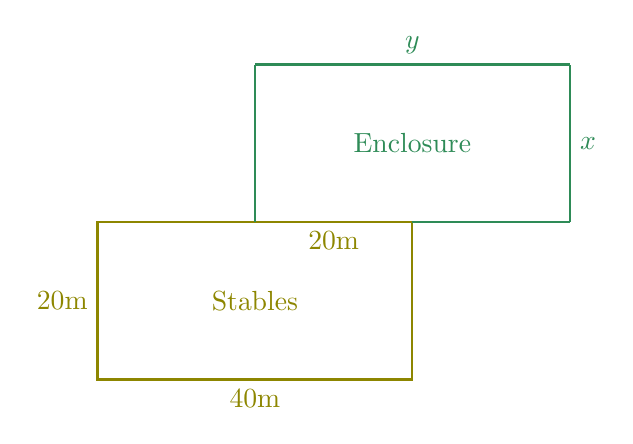
\begin{tikzpicture}
			\draw[color = olive, thick] (0,0) rectangle (4,2);
			\draw[color = SeaGreen, thick] (4,2) -- (6,2);
			\draw[color = SeaGreen, thick] (4,2) -- (6,2);
			\draw[color = SeaGreen, thick] (6,4) -- (2,4) node[midway, anchor = south] {$y$};
			\draw[color = SeaGreen, thick] (2,4) -- (2,2);
			\draw[color = SeaGreen, thick] (6,2) -- (6,4) node[midway, anchor = west] {$x$};
			\node[color = olive] at (2,1) {Stables};
			\node[color = SeaGreen] at (4,3) {Enclosure};
			\node[color = olive, anchor = north] at (2,0) {40m};
			\node[color = olive, anchor = east] at (0,1) {20m};
			\node[color = olive, anchor = north] at (3,2) {20m};
		\end{tikzpicture}
		\caption{Enclosure next to stables.}
		\label{fig:horse}
	\end{figure}
	\phantom{h}
\end{opgavetekst}
\begin{delopgave}{1}
	Determine an equation for the circumference of the enclosure.
\end{delopgave}
\begin{delopgave}{2}
	Determine the dimensions for the enclosure that maximises the area of the enclosure. 
\end{delopgave}